% https://texnique.fr/osqa/questions/6583/beamer-superposition-dimages/6584
\documentclass{beamer}
\usepackage{tikz}
\begin{document}
\begin{frame}
    \begin{figure}
    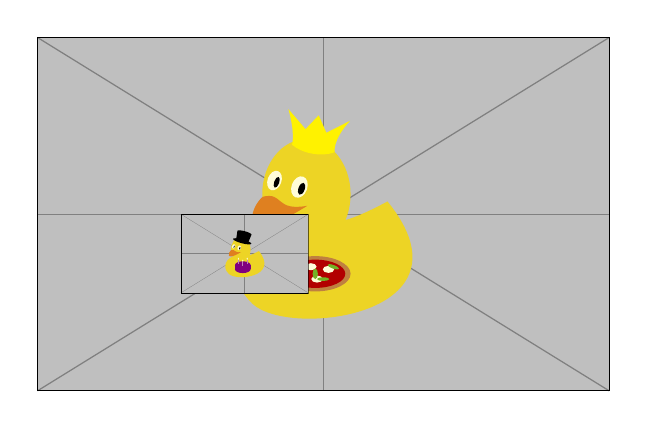
\begin{tikzpicture}
    \node at (0,0) {\includegraphics[width=.6\textwidth]{example-image-duck}};
    \node at (-1,-0.5) {\includegraphics[scale=0.25,page=2]{example-image-duck}};
    \end{tikzpicture}        
    \caption{blabla}
    \end{figure}
\end{frame}
\end{document}